\documentclass[9pt]{beamer}
\usetheme{cmepda}

\usepackage[utf8]{inputenc}
\usepackage[T1]{fontenc}


\title{Testing and documentation}
\subtitle{Computing Methods for Experimental Physics and Data Analysis}
\date{\today}
\author{L. Baldini}
\institute[UNIPI and INFN]{Universit\`a and INFN--Pisa}
\email{luca.baldini@pi.infn.it}


\begin{document}

\titleframe

%Documentation: sphinx, reStructuredText
%Making the docs available: readthedocs


\begin{frame}
  \frametitle{How do I make sure my program is correct?}
  \begin{itemize}
  \item The short answer is: in real life you don't!
    \begin{itemize}
    \item Especially if your code is asynchronous
    \end{itemize}
  \item \alert{That is not the same a saying there is nothing you can do}
  \item For compiled langauges the compiler will flag all obvious (and a whola
    lotta of non-obvious) mistakes
    \begin{itemize}
    \item This doesn't really apply to Python, since Python is interpreted
    \item Although the interpreter will stop upon syntax errors
    \end{itemize}
  \item Besides paying attention, there are two things that you can do even
    in interpreted languages:
    \begin{enumerate}
    \item \alert{Unit testing}
    \item \alert{Static analysis}
    \end{enumerate}
  \item Generally people hate both, but they should come right next to
    version control in your work-flow toolbox
  \end{itemize}
\end{frame}


\begin{frame}
  \frametitle{Unit testing na\"ive example}
  \begin{Verbatim}[label=\makebox{\url{https://github.com/lucabaldini/cmepda/tree/master/slides/latex/snippets/unit\_test\_naive.py}},commandchars=\\\{\}]
\PY{k}{def} \PY{n+nf}{square}\PY{p}{(}\PY{n}{x}\PY{p}{)}\PY{p}{:}
    \PY{l+s+sd}{\PYZdq{}\PYZdq{}\PYZdq{}Function returning the suare of x.}
\PY{l+s+sd}{    \PYZdq{}\PYZdq{}\PYZdq{}}
    \PY{k}{return} \PY{n}{x}\PY{o}{*}\PY{o}{*}\PY{l+m+mf}{2.}

\PY{k}{def} \PY{n+nf}{test}\PY{p}{(}\PY{p}{)}\PY{p}{:}
    \PY{l+s+sd}{\PYZdq{}\PYZdq{}\PYZdq{}Dumb unit test\PYZhy{}\PYZhy{}\PYZhy{}make sure that the square of 2. is 4.}
\PY{l+s+sd}{    \PYZdq{}\PYZdq{}\PYZdq{}}
    \PY{k}{assert} \PY{n}{square}\PY{p}{(}\PY{l+m+mf}{2.}\PY{p}{)} \PY{o}{==} \PY{l+m+mf}{4.}
    \PY{k}{print}\PY{p}{(}\PY{l+s+s1}{\PYZsq{}}\PY{l+s+s1}{Passed\PYZhy{}\PYZhy{}\PYZhy{}cool!}\PY{l+s+s1}{\PYZsq{}}\PY{p}{)}


\PY{k}{if} \PY{n+nv+vm}{\PYZus{}\PYZus{}name\PYZus{}\PYZus{}} \PY{o}{==} \PY{l+s+s1}{\PYZsq{}}\PY{l+s+s1}{\PYZus{}\PYZus{}main\PYZus{}\PYZus{}}\PY{l+s+s1}{\PYZsq{}}\PY{p}{:}
    \PY{n}{test}\PY{p}{(}\PY{p}{)}

[Output]
Passed---cool!
\end{Verbatim}
\end{frame}


\begin{frame}
  \frametitle{Unit testing in a nutshell}
  \begin{itemize}
  \item Break up your program in many small pieces
    \begin{itemize}
    \item Each piece should encapsulate a well-defined and (possibly) simple
      functionality
    \end{itemize}
  \item This is usually accomplished by means of a sensible hierarchy of
    functions and classes
    \begin{itemize}
    \item And this is typically the hardest task when structuring your code
    \item And the code will evolve with time, so you will find yourself
      \alert{refactoring code} from time to time
    \item Remember to be dry: don't repeat youself
    \end{itemize}
  \item \alert{Unit testing is: make sure that each single piece is
    correct by implementing a series of basic checks}
    \begin{itemize}
    \item You know what each elementary piece of code is suppose to be
    \item Make sure it does
    \item And make sure it does with any valid input
    \end{itemize}
  \item This is much simpler that testing the whole program at once
    \begin{itemize}
    \item Although you have to do that, too
    \end{itemize}
  \item \alert{Test-Driven Development (TDD)}
    \begin{enumerate}
    \item Write an empty placeholder for your new function
    \item Write all the unit tests (they will fail)
    \item Implement your function and tweak it until all the tests pass
    \end{enumerate}
  \end{itemize}
\end{frame}


\begin{frame}
  \frametitle{Back to our na\"ive example}
  \begin{Verbatim}[label=\makebox{\url{https://github.com/lucabaldini/cmepda/tree/master/slides/latex/snippets/unit\_test\_naive.py}},commandchars=\\\{\}]
\PY{k}{def} \PY{n+nf}{square}\PY{p}{(}\PY{n}{x}\PY{p}{)}\PY{p}{:}
    \PY{l+s+sd}{\PYZdq{}\PYZdq{}\PYZdq{}Function returning the suare of x.}
\PY{l+s+sd}{    \PYZdq{}\PYZdq{}\PYZdq{}}
    \PY{k}{return} \PY{n}{x}\PY{o}{*}\PY{o}{*}\PY{l+m+mf}{2.}

\PY{k}{def} \PY{n+nf}{test}\PY{p}{(}\PY{p}{)}\PY{p}{:}
    \PY{l+s+sd}{\PYZdq{}\PYZdq{}\PYZdq{}Dumb unit test\PYZhy{}\PYZhy{}\PYZhy{}make sure that the square of 2. is 4.}
\PY{l+s+sd}{    \PYZdq{}\PYZdq{}\PYZdq{}}
    \PY{k}{assert} \PY{n}{square}\PY{p}{(}\PY{l+m+mf}{2.}\PY{p}{)} \PY{o}{==} \PY{l+m+mf}{4.}
    \PY{k}{print}\PY{p}{(}\PY{l+s+s1}{\PYZsq{}}\PY{l+s+s1}{Passed\PYZhy{}\PYZhy{}\PYZhy{}cool!}\PY{l+s+s1}{\PYZsq{}}\PY{p}{)}


\PY{k}{if} \PY{n+nv+vm}{\PYZus{}\PYZus{}name\PYZus{}\PYZus{}} \PY{o}{==} \PY{l+s+s1}{\PYZsq{}}\PY{l+s+s1}{\PYZus{}\PYZus{}main\PYZus{}\PYZus{}}\PY{l+s+s1}{\PYZsq{}}\PY{p}{:}
    \PY{n}{test}\PY{p}{(}\PY{p}{)}

[Output]
Passed---cool!
\end{Verbatim}

  \medskip
  
  \begin{itemize}    
  \item This is fine, but everything happens manually
    \begin{itemize}
    \item You have to run the script yourself
    \item You have to inspect the output yourself
    \end{itemize}
  \item As your code grows in complexity, this is not very effective
  \end{itemize}
\end{frame}


\begin{frame}
  \frametitle{Unit tests the Python way}
  \framesubtitle{The unittest module}
  \begin{Verbatim}[label=\makebox{\url{https://github.com/lucabaldini/cmepda/tree/master/slides/latex/snippets/unit\_test.py}},commandchars=\\\{\}]
\PY{k+kn}{import} \PY{n+nn}{unittest}

\PY{k}{def} \PY{n+nf}{square}\PY{p}{(}\PY{n}{x}\PY{p}{)}\PY{p}{:}
    \PY{l+s+sd}{\PYZdq{}\PYZdq{}\PYZdq{}Function returning the suare of x.}

\PY{l+s+sd}{    In real life this would be in a differnt module!}
\PY{l+s+sd}{    \PYZdq{}\PYZdq{}\PYZdq{}}
    \PY{k}{return} \PY{n}{x}\PY{o}{*}\PY{o}{*}\PY{l+m+mf}{2.}


\PY{k}{class} \PY{n+nc}{TestSquare}\PY{p}{(}\PY{n}{unittest}\PY{o}{.}\PY{n}{TestCase}\PY{p}{)}\PY{p}{:}

    \PY{k}{def} \PY{n+nf}{test}\PY{p}{(}\PY{n+nb+bp}{self}\PY{p}{)}\PY{p}{:}
        \PY{l+s+sd}{\PYZdq{}\PYZdq{}\PYZdq{}Dumb unit test\PYZhy{}\PYZhy{}\PYZhy{}make sure that the square of 2. is 4.}
\PY{l+s+sd}{        \PYZdq{}\PYZdq{}\PYZdq{}}
        \PY{n+nb+bp}{self}\PY{o}{.}\PY{n}{assertAlmostEqual}\PY{p}{(}\PY{n}{square}\PY{p}{(}\PY{l+m+mf}{2.}\PY{p}{)}\PY{p}{,} \PY{l+m+mf}{4.}\PY{p}{)}


\PY{k}{if} \PY{n+nv+vm}{\PYZus{}\PYZus{}name\PYZus{}\PYZus{}} \PY{o}{==} \PY{l+s+s1}{\PYZsq{}}\PY{l+s+s1}{\PYZus{}\PYZus{}main\PYZus{}\PYZus{}}\PY{l+s+s1}{\PYZsq{}}\PY{p}{:}
    \PY{n}{unittest}\PY{o}{.}\PY{n}{main}\PY{p}{(}\PY{p}{)}

[Output]
.
----------------------------------------------------------------------
Ran 1 test in 0.000s

OK
\end{Verbatim}
\end{frame}


\begin{frame}
  \frametitle{Wait a moment\ldots}
  \framesubtitle{How is this different?}
  \begin{itemize}
  \item This is much better!
  \item The base TestCase class offers all the goodies for unit testing
    \begin{itemize}
    \item assertTrue(), assertFalse(), assertEqual(), assertAlmostEqual()\ldots
    \end{itemize}
  \item The execution can be easily made automatic:
    \begin{itemize}
    \item Put all your unit test modules into a test folder
    \item Run \texttt{python -m unittest discover}
    \item (Or, even better, write a small Makefile or .bat script to do that)
    \item That's it---all your tests are run in sequence
    \end{itemize}
  \item Did you just find a bug in your code?
    \begin{itemize}
    \item Make sure you add a unit test along with the fix, so that you'll
      never be hurt again by that particular bug
    \end{itemize}
  \item Are you adding a new feature?
    \begin{itemize}
    \item Make sure the new code is covered by unit tests
    \item You should not be obsessed by the coverage, but you should
      definitely aim for it to be as large as possible
    \end{itemize}
  \item \alert{You should always make sure that all the unit tests are
    passing before merging stuff on the master}    
  \item More about this in a bit (we'll be talking about continuous integration)
  \end{itemize}
\end{frame}


\begin{frame}
  \frametitle{Static code analysis}
  \begin{itemize}
  \item By its very nature, Python will show you all the errors at runtime
  \item Say you have a bug in a part of the code that is exercised very rarely,
    and not covered by unit tests
    \begin{itemize}
    \item Python might crash the first time you exercise it\ldots
    \item or Python might happily do \emph{something} that is not what you
      intended
    \end{itemize}
  \item \alert{It might take years for even realizing that there is a bug}
  \item Many common mistakes can be found by just looking at the code
    \begin{itemize}
    \item And in fact all of them can, at least in principle
    \end{itemize}
  \item Part of it can be done programmatically
    \begin{itemize}
    \item Generally, a program will not \emph{understand} your program
    \item But a program can be trained to spot some kind of
      errors and inconsistencies
    \end{itemize}
  \item Pylint and pyflakes are good examples of such tools
  \end{itemize}
\end{frame}


\begin{frame}[fragile]
  \frametitle{Static analysis: an example}
  \begin{Verbatim}[label=\makebox{\url{https://github.com/lucabaldini/cmepda/tree/master/slides/latex/snippets/linting1.py}},commandchars=\\\{\}]
\PY{n}{x} \PY{o}{=} \PY{l+m+mf}{1.}
\PY{n}{y} \PY{o}{=} \PY{l+m+mf}{2.}
\PY{n}{very\PYZus{}uncommon\PYZus{}condition} \PY{o}{=} \PY{n+nb+bp}{False}
\PY{k}{if} \PY{n}{very\PYZus{}uncommon\PYZus{}condition}\PY{p}{:}
    \PY{k}{print}\PY{p}{(}\PY{n}{x} \PY{o}{+} \PY{n}{z}\PY{p}{)}
\PY{k}{else}\PY{p}{:}
    \PY{k}{print}\PY{p}{(}\PY{n}{x} \PY{o}{+} \PY{n}{y}\PY{p}{)}

[Output]
3.0
\end{Verbatim}

  \smallskip
  \begin{itemize}
  \item And here is the pylint output
  \end{itemize}
  \smallskip

  {\scriptsize
    \begin{Verbatim}
[lbaldini@nbbaldini latex]$ pylint snippets/linting1.py 
************* Module snippets.linting1
snippets/linting1.py:1:0: C0111: Missing module docstring (missing-docstring)
snippets/linting1.py:1:0: C0103: Constant name "x" doesn't conform to UPPER_CASE
                          naming style (invalid-name)
snippets/linting1.py:2:0: C0103: Constant name "y" doesn't conform to UPPER_CASE
                          naming style (invalid-name)
snippets/linting1.py:3:0: C0103: Constant name "very_uncommon_condition" doesn't
                          conform to UPPER_CASE naming style (invalid-name)
snippets/linting1.py:5:14: E0602: Undefined variable 'z' (undefined-variable)

--------------------------------------------------------------------
Your code has been rated at -5.00/10 (previous run: -5.00/10, +0.00)
    \end{Verbatim}
  }
\end{frame}


\begin{frame}
  \frametitle{Static code analysis}
  \begin{itemize}
  \item \alert{You should consider using static code analysis routinely}
  \item Static analysis tools tend to be quite verbose
    \begin{itemize}
    \item And often times verbose is the same as annoying
    \end{itemize}
  \item They try and enforce many different (good!) things at once
    \begin{itemize}
    \item Formal correctness
    \item Efficiency
    \item Avoiding anti-patterns
    \item Style guides
    \item Generic conventions
    \end{itemize}
  \item They also are typically highly customizable
    \begin{itemize}
    \item i.e., you can mute errors you don't care about
    \item But be advised: you most of the times you should probably care
    \end{itemize}
  \item \alert{Finding a good balance is generally not too hard}
  \item And trust me: it will help you in the long run
  \end{itemize}
\end{frame}


\begin{frame}
  \frametitle{Digression: optional static typing in Python}
  \begin{Verbatim}[label=\makebox{\url{https://github.com/lucabaldini/cmepda/tree/master/slides/latex/snippets/type\_annotation.py}},commandchars=\\\{\}]
\PY{k}{def} \PY{n+nf}{square}\PY{p}{(}\PY{n}{x}\PY{p}{)}\PY{p}{:}
    \PY{l+s+sd}{\PYZdq{}\PYZdq{}\PYZdq{}Return the square of a number.}
\PY{l+s+sd}{    \PYZdq{}\PYZdq{}\PYZdq{}}
    \PY{k}{return} \PY{n}{x}\PY{o}{*}\PY{o}{*}\PY{l+m+mf}{2.}

\PY{k}{def} \PY{n+nf}{annotated\PYZus{}square}\PY{p}{(}\PY{n}{x}\PY{p}{:} \PY{n+nb}{float}\PY{p}{)} \PY{o}{\PYZhy{}}\PY{o}{\PYZgt{}} \PY{n+nb}{float}\PY{p}{:}
    \PY{l+s+sd}{\PYZdq{}\PYZdq{}\PYZdq{}Return the square of a number.}
\PY{l+s+sd}{    \PYZdq{}\PYZdq{}\PYZdq{}}
    \PY{k}{return} \PY{n}{x}\PY{o}{*}\PY{o}{*}\PY{l+m+mf}{2.}

\PY{k}{print}\PY{p}{(}\PY{n}{square}\PY{p}{(}\PY{l+m+mf}{2.}\PY{p}{)}\PY{p}{)}
\PY{k}{print}\PY{p}{(}\PY{n}{annotated\PYZus{}square}\PY{p}{(}\PY{l+m+mf}{2.}\PY{p}{)}\PY{p}{)}

[Output]
4.0
4.0
\end{Verbatim}
  
  \begin{itemize}
  \item Recent Python 3 versions support type annotations
  \item \alert{The Python interpreter recognizes but does nothing with
    annotations}
    \begin{itemize}
    \item And so what?
    \end{itemize}
  \item Well\ldots they are handy (as comments are)
    \begin{itemize}
    \item The code is easier to read
    \item Even more checks wrt un-annotated code can be done by tools such as
      mypy
    \end{itemize}
  \end{itemize}
\end{frame}


\begin{frame}
  \frametitle{Continuous integration}
  \begin{itemize}
  \item Imagine for a second\ldots
    \begin{itemize}
    \item Wouldn't it be nice if sombody run all the unit tests of my
      package every time I push on the master or make a pull request?
    \item And, since we are at it, sent me an email if any of the tests fail?
    \end{itemize}
  \item \ldots Well, such a thing exists and it is standard practice in
    code dvelopment
  \item People even made a name for it: \alert{Continuous Integration (CI)}
  \item CI cloud-base services exists just like code-hostng services exist
    \begin{itemize}
    \item Travis-CI and circleci are two good examples
    \end{itemize}
  \item They interoperates seamlessly with github, gitlab or bitbucket
  \item Setting up CI for your package is usually fairly simple
  \item \alert{One-sentence summary: go ahead and do it. Always.}
  \end{itemize}
\end{frame}


\begin{frame}
  \frametitle{One last thing: documentation}
  \framesubtitle{How do the hell they do that?}
  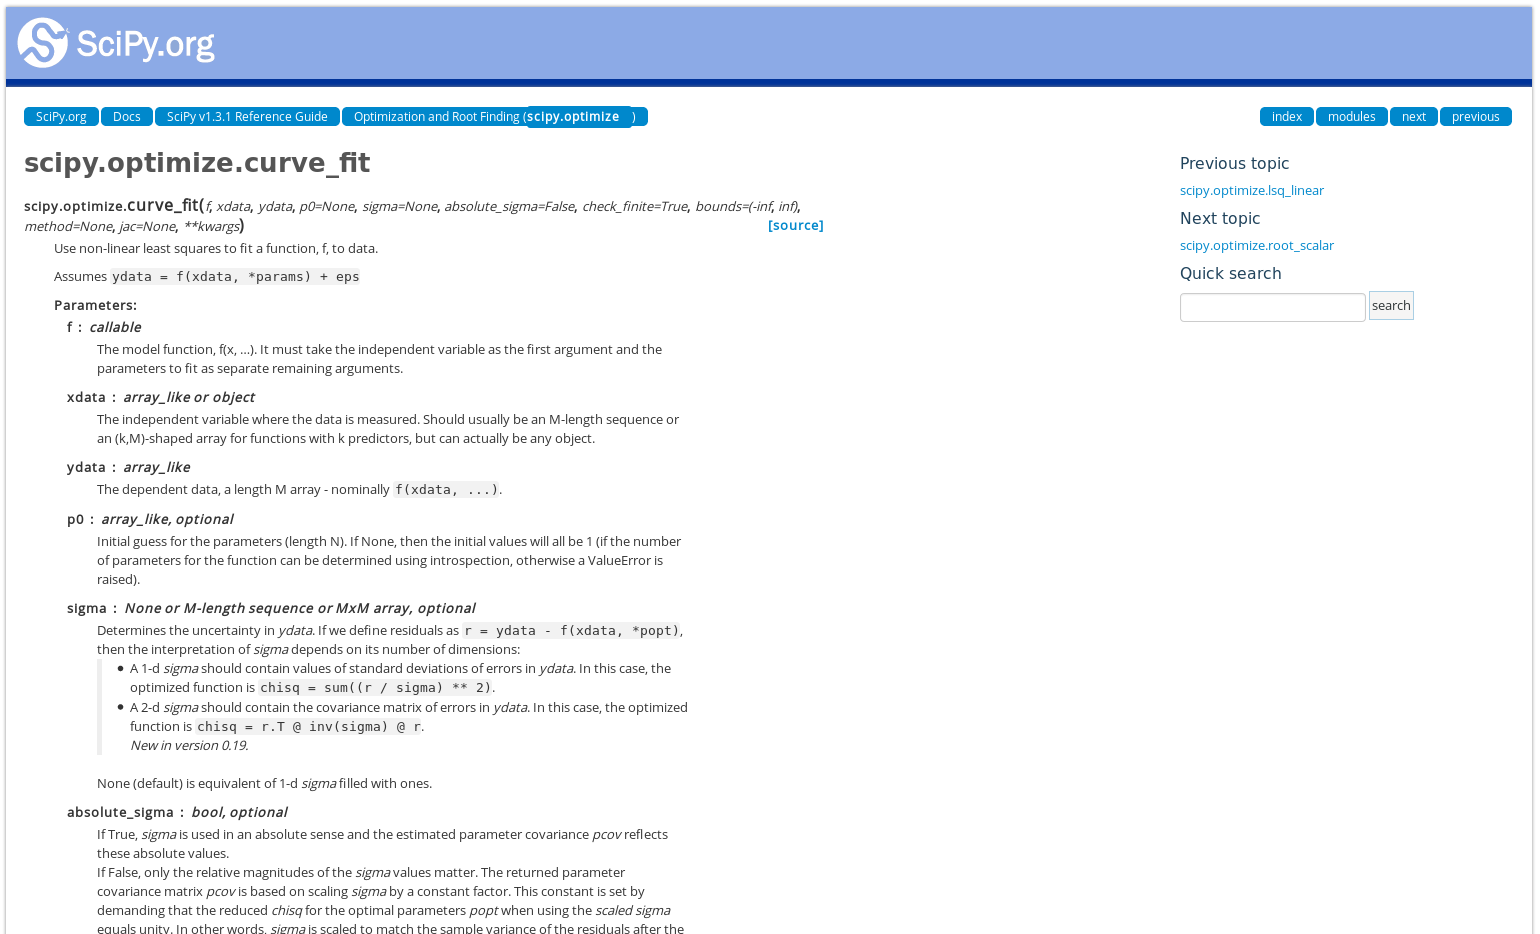
\includegraphics[width=\textwidth]{curve_fit_docs}
\end{frame}


\begin{frame}
  \frametitle{One last thing: documentation}
  \framesubtitle{Ah---the documentation is embedded in the code\ldots}
  \centering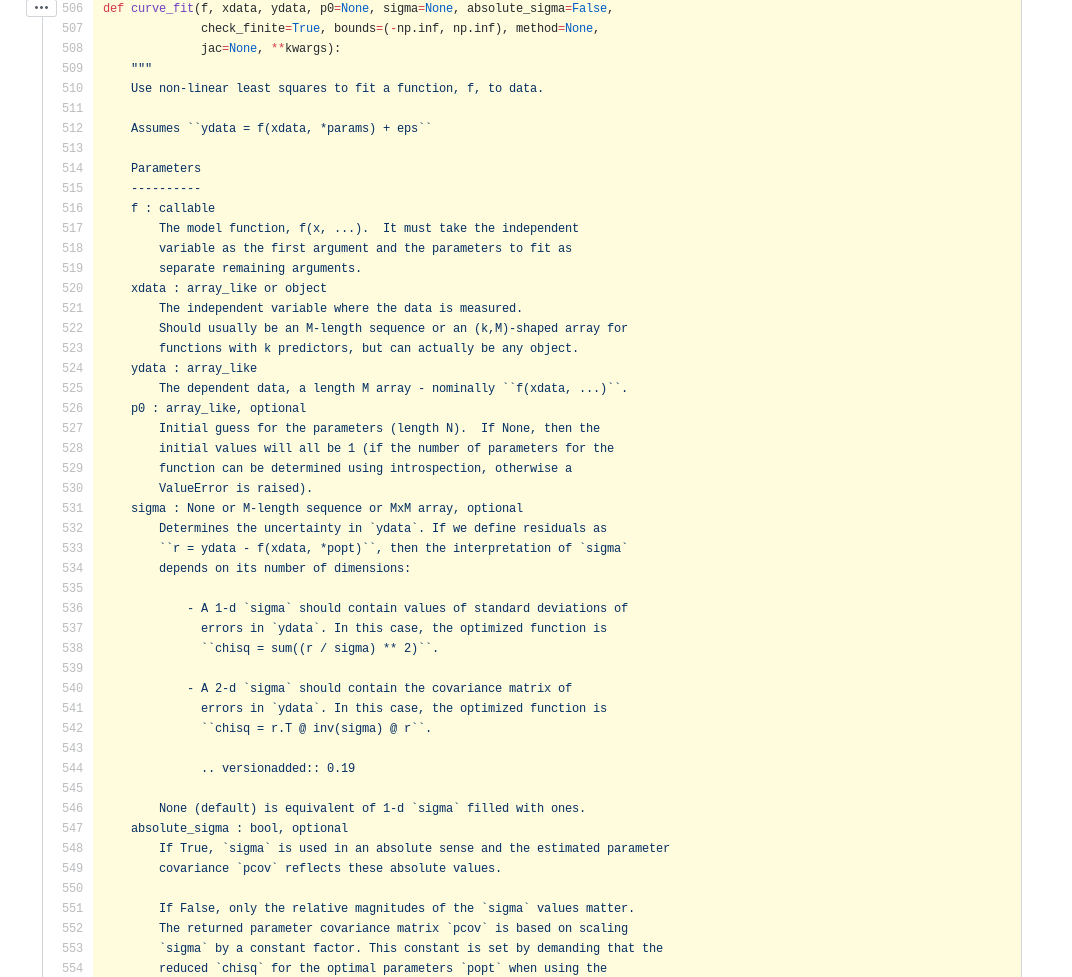
\includegraphics[width=0.75\textwidth]{curve_fit_code}
  
\end{frame}


\begin{frame}
  \frametitle{Sphinx: the documentation tool for Python}
  \centering
\includegraphics[width=0.85\textwidth]{sphinx}
  
\end{frame}


\begin{frame}
  \frametitle{Sphinx basics}
  \begin{itemize}
  \item Process all the relevant information to produce several types of
    output
    \begin{itemize}
    \item Most notably html and LaTeX
    \end{itemize}
  \item Two different sources:
    \begin{enumerate}
    \item The doctrings in the Python modules
    \item Additional markup files (in reStructuredText) containing
      auxiliary information
    \end{enumerate}
  \item Typical workflow:
    \begin{itemize}
    \item Use \texttt{sphinx-quickstart} once when you setup your project
    \item Tweak the generated \texttt{conf.py} file to suit your needs
    \item Go ahead and have fun!
    \end{itemize}
  \item Sphinx is \emph{very} powerful
    \begin{itemize}
    \item e.g., \url{https://docs.python-guide.org/} is written in Sphinx,
      and so is all the Python documentation
    \end{itemize}
  \end{itemize}
\end{frame}


\begin{frame}
  \frametitle{Ok, I have the documentation compiled}
  \framesubtitle{Now what do I do with it?}
  \begin{itemize}
  \item Wouldn't it be nice if the documentation was automatically compiled and
    uploaded on the web each time I push on the master?
  \item This is possible and is called readthedocs.com
    \begin{itemize}
    \item And, again, this is a cloud-based service that can interoperate
      easily with github, gitlab or bitbucket
    \end{itemize}
  \end{itemize}
\end{frame}


\begin{frame}
  \frametitle{References}
  \scriptsize
  \begin{itemize}
  \item \url{https://docs.python.org/3/library/unittest.html}
  \item \url{https://www.pylint.org/}
  \item \url{https://pypi.org/project/pyflakes/}
  \item \url{http://mypy-lang.org/}
  \item \url{https://circleci.com/}
  \item \url{https://travis-ci.org/}
  \item \url{http://www.sphinx-doc.org/en/master/}
  \end{itemize}
\end{frame}


\end{document}
